
\documentclass[12pt]{amsart}
\usepackage{listings}
\usepackage{color}
\usepackage{graphicx}
\usepackage{palatino}
\usepackage{tikz}
\usepackage{amssymb}
\usepackage{cite}
\usepackage[colorlinks,linkcolor=red]{hyperref}
\usetikzlibrary{shapes.geometric, arrows}

\definecolor{dkgreen}{rgb}{0,0.6,0}
\definecolor{gray}{rgb}{0.5,0.5,0.5}
\definecolor{mauve}{rgb}{0.58,0,0.82}

\lstset{frame=tb,
  language=Python,
  aboveskip=3mm,
  belowskip=3mm,
  showstringspaces=false,
  columns=flexible,
  basicstyle={\small\ttfamily},
  numbers=none,
  numberstyle=\tiny\color{gray},
  keywordstyle=\color{blue},
  commentstyle=\color{dkgreen},
  stringstyle=\color{mauve},
  breaklines=true,
  breakatwhitespace=true,
  tabsize=3
}
\title{NLP_HW3}
\author{Xuan Wang}
\date{} % delete this line to display the current date

%%% BEGIN DOCUMENT

\begin{document}


\begin{titlepage}

\begin{center}


% Upper part of the page

\textsc{\LARGE University of Rutgers}\\[1.5cm]

\textsc{\Large Assignment 1: Fast Trajectory Planning}\\[0.5cm]


% Author and supervisor
\begin{minipage}{0.4\textwidth}
\begin{flushleft} \large
\emph{Author:}\\
Xuan \textsc{Wang}

Xunjie \textsc{Zhu}
\end{flushleft}
\end{minipage}
\begin{minipage}{0.4\textwidth}
\begin{flushright} \large
\emph{Supervisor:} \\
Abdeslam  \textsc{Boularias}
\end{flushright}
\end{minipage}

\vfill

% Bottom of the page
{\large \today}

\end{center}

\end{titlepage}

%\section*{Part 0}
%For the maze, define a maze class, use \emph{numpy} external library to generate a 2-d 101*101 int array representing the maze. Then use \emph{networkx} library to convert the maze into an undirected graph by adding edges for each pair of adjacency nodes, use \emph{dfs\_preorder\_nodes()} method to find a traverse list by DFS, for each visited node make it blocked of 30\% chance
%\begin{lstlisting}
%self.array = np.zeros((m,n))
%traverselist = list(nx.dfs_preorder_nodes(self.graph,(0,0)))
%p_list = [1,1,1,0,0,0,0,0,0,0]
%traverselist = self.DFS()
%for i in traverselist:
%	self.array[i[0],i[1]] = random.choice(p_list)
%\end{lstlisting}
%The following picture is a visualization implement by scala
%
%
%\newpage
%%%%%%%%%%%%%%%%%%%%%%%%%%%%%%%%%%%%%%%%%
% University/School Laboratory Report
% LaTeX Template
% Version 3.1 (25/3/14)
%
% This template has been downloaded from:
% http://www.LaTeXTemplates.com
%
% Original author:
% Linux and Unix Users Group at Virginia Tech Wiki 
% (https://vtluug.org/wiki/Example_LaTeX_chem_lab_report)
%
% License:
% CC BY-NC-SA 3.0 (http://creativecommons.org/licenses/by-nc-sa/3.0/)
%
%%%%%%%%%%%%%%%%%%%%%%%%%%%%%%%%%%%%%%%%%

%----------------------------------------------------------------------------------------
%	PACKAGES AND DOCUMENT CONFIGURATIONS
%----------------------------------------------------------------------------------------

\documentclass{article}

\usepackage[version=3]{mhchem} % Package for chemical equation typesetting
\usepackage{siunitx} % Provides the \SI{}{} and \si{} command for typesetting SI units
\usepackage{graphicx} % Required for the inclusion of images
\usepackage{amsmath} % Required for some math elements 
\usepackage{caption}
\usepackage{amssymb}
\setlength\parindent{0pt} % Removes all indentation from paragraphs

\renewcommand{\labelenumi}{\alph{enumi}.} % Make numbering in the enumerate environment by letter rather than number (e.g. section 6)

%\usepackage{times} % Uncomment to use the Times New Roman font

%----------------------------------------------------------------------------------------
%	DOCUMENT INFORMATION
%----------------------------------------------------------------------------------------

\title{Assignment 3} % Title

\author{Xunjie \textsc{Zhu}  \& Xuan \textsc{Wang}} % Author name
\date{\today} % Date for the report

\begin{document}

\maketitle % Insert the title, author and date

\begin{center}
\begin{tabular}{l r}
Date Performed: & February 24 - March 1 , 2017 \\ % Date the experiment was performed
\end{tabular}
\end{center}

% If you wish to include an abstract, uncomment the lines below
% \begin{abstract}
% Abstract text
% \end{abstract}

%----------------------------------------------------------------------------------------
%	SECTION 1
%----------------------------------------------------------------------------------------



%----------------------------------------------------------------------------------------
%	SECTION 1
%----------------------------------------------------------------------------------------

\section*{Problem 3}
Enforce arc-consistency for the following problem

Two constraints $C(x,y)$ and $C(y,z)$

For $C(x,y)$

$x=[6,10]$ removed

Add $C(y,x)$

For $C(y,x)$

$y=[10,15]$ removed

For $C(z,y)$

$z=[-1,10]$ removed

Add $C(y,z)$

For $C(y,z)$

$revise=false$

And it is arc consistent where $dom(x)=[1,5], dom(y)=[5,9], dom(z)=[-10,-2]$

\section*{Problem 5}
(a)Apply variable elimination to the query

$P(B=true|J=ture,M=true)=\alpha\sum\limits_{E,A}P(B=true,E,A,J=true,M=true)$

$P(B=true|J=ture,M=true)=\alpha\sum\limits_{E,A}(P(B=true)P(E)P(A|B=true,E)P(J=true|A)P(M=true|A))$

Sum out

$P(B=true|J=ture,M=true)=\alpha P(B=true)\sum\limits_{E}P(E)\sum\limits_{A}P(A|B=true,E)P(J=true|A)P(M=true|A)$

$P(B=true|J=ture,M=true)=\alpha P(B=true)\sum\limits_{E}P(E)f_{\overline{A}JM}(B=true,E)$

Where

$f_{\overline{A}JM}(B=true,E=true)=0.9*0.7*0.95+0.05*0.01*0.05=0.598525$ and $f_{\overline{A}JM}(B=true,E=false)=0.9*0.7*0.94+0.05*0.01*0.06=0.59223$

Continuing,

$P(B=true|J=ture,M=true)=\alpha P(B=true)f_{\overline{EA}JM}(B=true,E)$

Where

$f_{\overline{EA}JM}(B=true)=0.598525*0.002+0.59223*0.998=0.59224259$

Continuing,

$P(B=true|J=ture,M=true)=\alpha 0.001*0.59224259=0.00059224259\alpha$

We can compute $P(B=false|J=ture,M=true)$ the same

$P(B=false|J=ture,M=true)=\alpha\sum\limits_{E,A}P(B=false,E,A,J=true,M=true)$

$P(B=false|J=ture,M=true)=\alpha\sum\limits_{E,A}(P(B=false)P(E)P(A|B=false,E)P(J=true|A)P(M=true|A))$

$P(B=false|J=ture,M=true)=\alpha P(B=false)\sum\limits_{E}P(E)\sum\limits_{A}P(A|B=false,E)P(J=true|A)P(M=true|A)$

$P(B=false|J=ture,M=true)=\alpha P(B=false)\sum\limits_{E}P(E)f_{\overline{A}JM}(B=false,E)$

Where

$f_{\overline{A}JM}(B=false,E=true)=0.9*0.7*0.29+0.05*0.01*0.71=0.183055$ and $f_{\overline{A}JM}(B=false,E=false)=0.9*0.7*0.001+0.05*0.01*0.999= 0.0011295$

Continuing,

$P(B=false|J=ture,M=true)=\alpha P(B=false)f_{\overline{EA}JM}(B=false,E)$

Where

$f_{\overline{EA}JM}(B=false)=0.183055*0.002+0.0011295*0.998=0.001493351$

Continuing,

$P(B=false|J=ture,M=true)=\alpha 0.999*0.001493351=0.001491857649\alpha$

So,%0.002084100239 0.28417183536439 0.71582816463561

$P(B=true|J=ture,M=true)=\frac{0.00059224259\alpha}{0.00059224259\alpha+0.001491857649\alpha}=0.28417$ $P(B=false|J=ture,M=true)=1-0.28417=0.71583$


%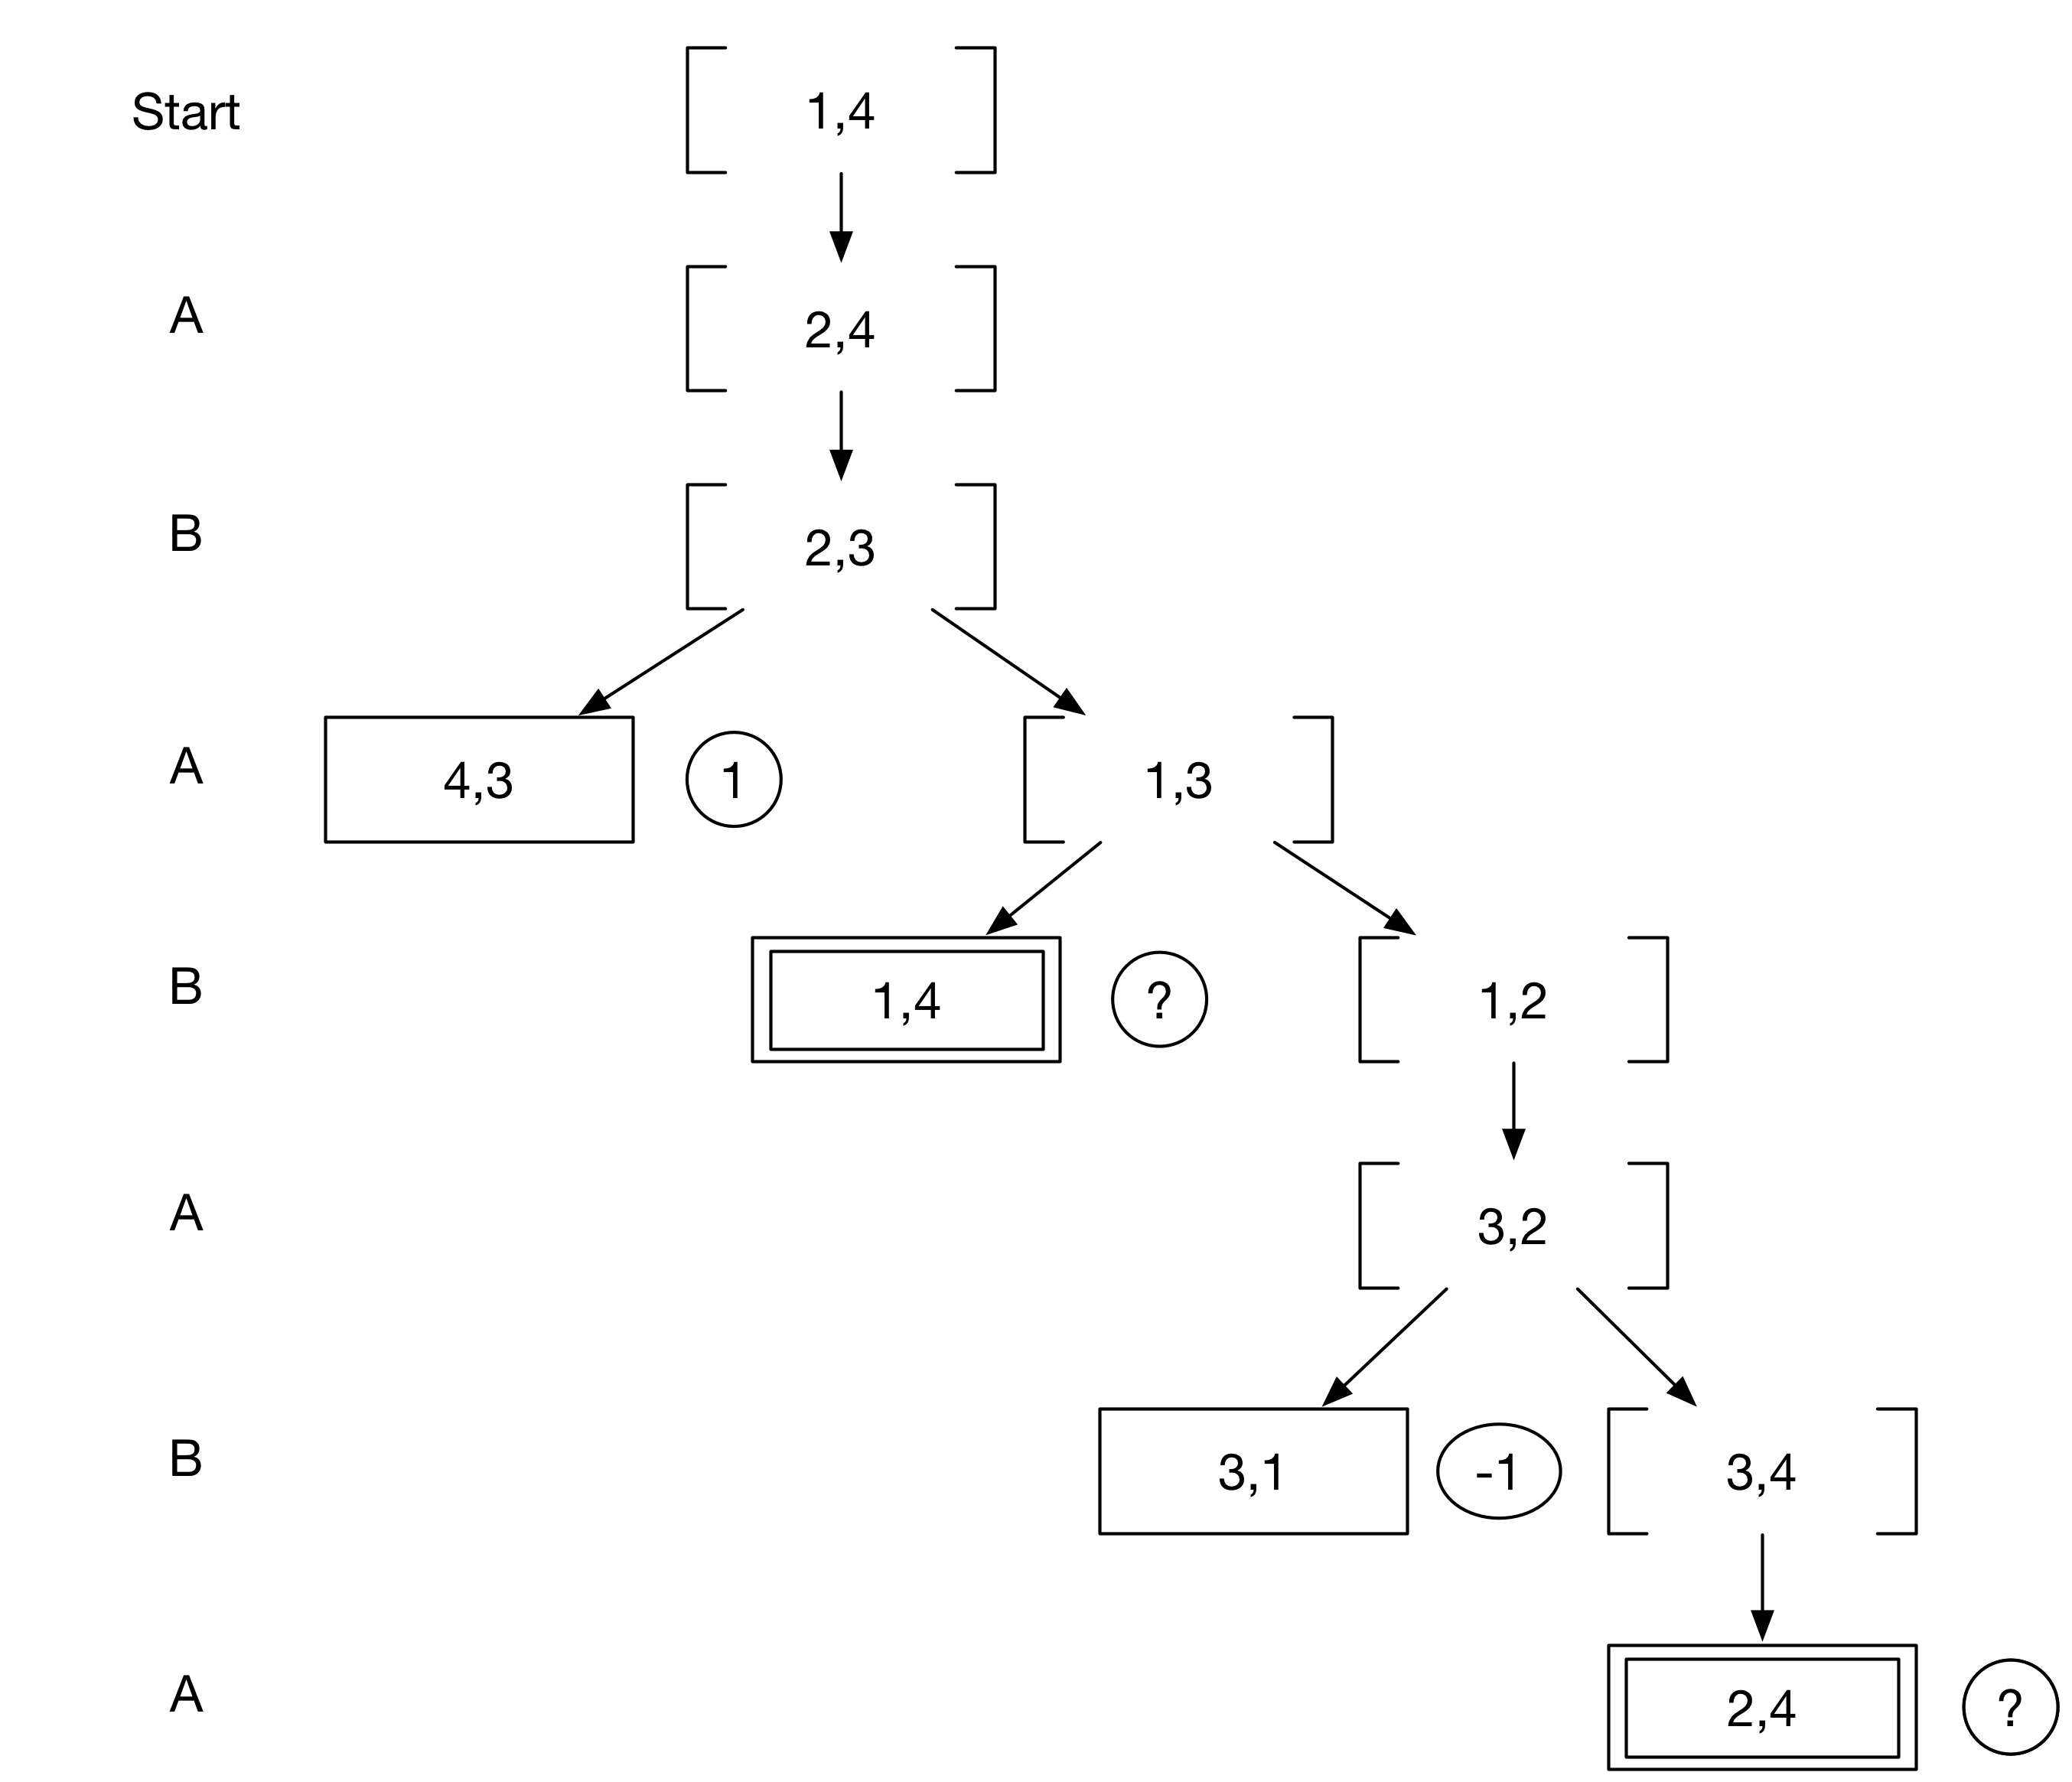
\includegraphics[width=\textwidth]{Problem4a.png}

\newpage
(b)Count the number of arithmetic operations

(1) variable elimination

$(0.9*0.7*0.95+0.05*0.01*0.05)*0.002+(0.9*0.7*0.94+0.05*0.01*0.06)*0.001$ takes 11 multiplications, 3 additions

There are two conditions $B=true,B=false$, so the operations are $14*2=28$

Final computation costs 1 substraction, 1 division, 1 addition

The total operations $28+3=31$

(2) enumeration

$P(B=false)P(E)P(A|B=false,E)P(J=true|A)P(M=true|A)$ takes 4 multiplications

$\sum\limits_{E,A}(P(B=false)P(E)P(A|B=false,E)P(J=true|A)P(M=true|A))$ takes $4*4=16$ multiplications and 3 additions

There are two conditions $B=true,B=false$, so the operations are $19*2=38$

Final computation costs 1 substraction, 1 division, 1 addition

The total operations $38+3=41$

(c) A Bayesian network has the from of a chain

(1) enumeration

$P(X_1|X_n=true)=\alpha \sum\limits_{{X_2}...{X_n-1}}P(X_1)P(X_2|X_1)...P(X_n|X_{n-1})$

There are $2^{n-2}$ choices for ${X_2}...{X_n-1}$, and each choice takes $n-1$ multiplications

So emumeration takes $O(n2^{n-2})$ time

(2) variable elimination

$P(X_1|X_n=true)=\alpha \sum\limits_{{X_2}}P(X_3|X_2)P(X_1)P(X_2|X_1)\sum\limits_{{X_3}}P(X_4|X_3)...\sum\limits_{{X_{n-1}}}P(X_n|X_{n-1})$

It takes $(n-2)*2$ additions and $n-2$ multiplications
So variable elimination takes $O(n)$ time
\newpage
\section*{Problem 7}

(a)

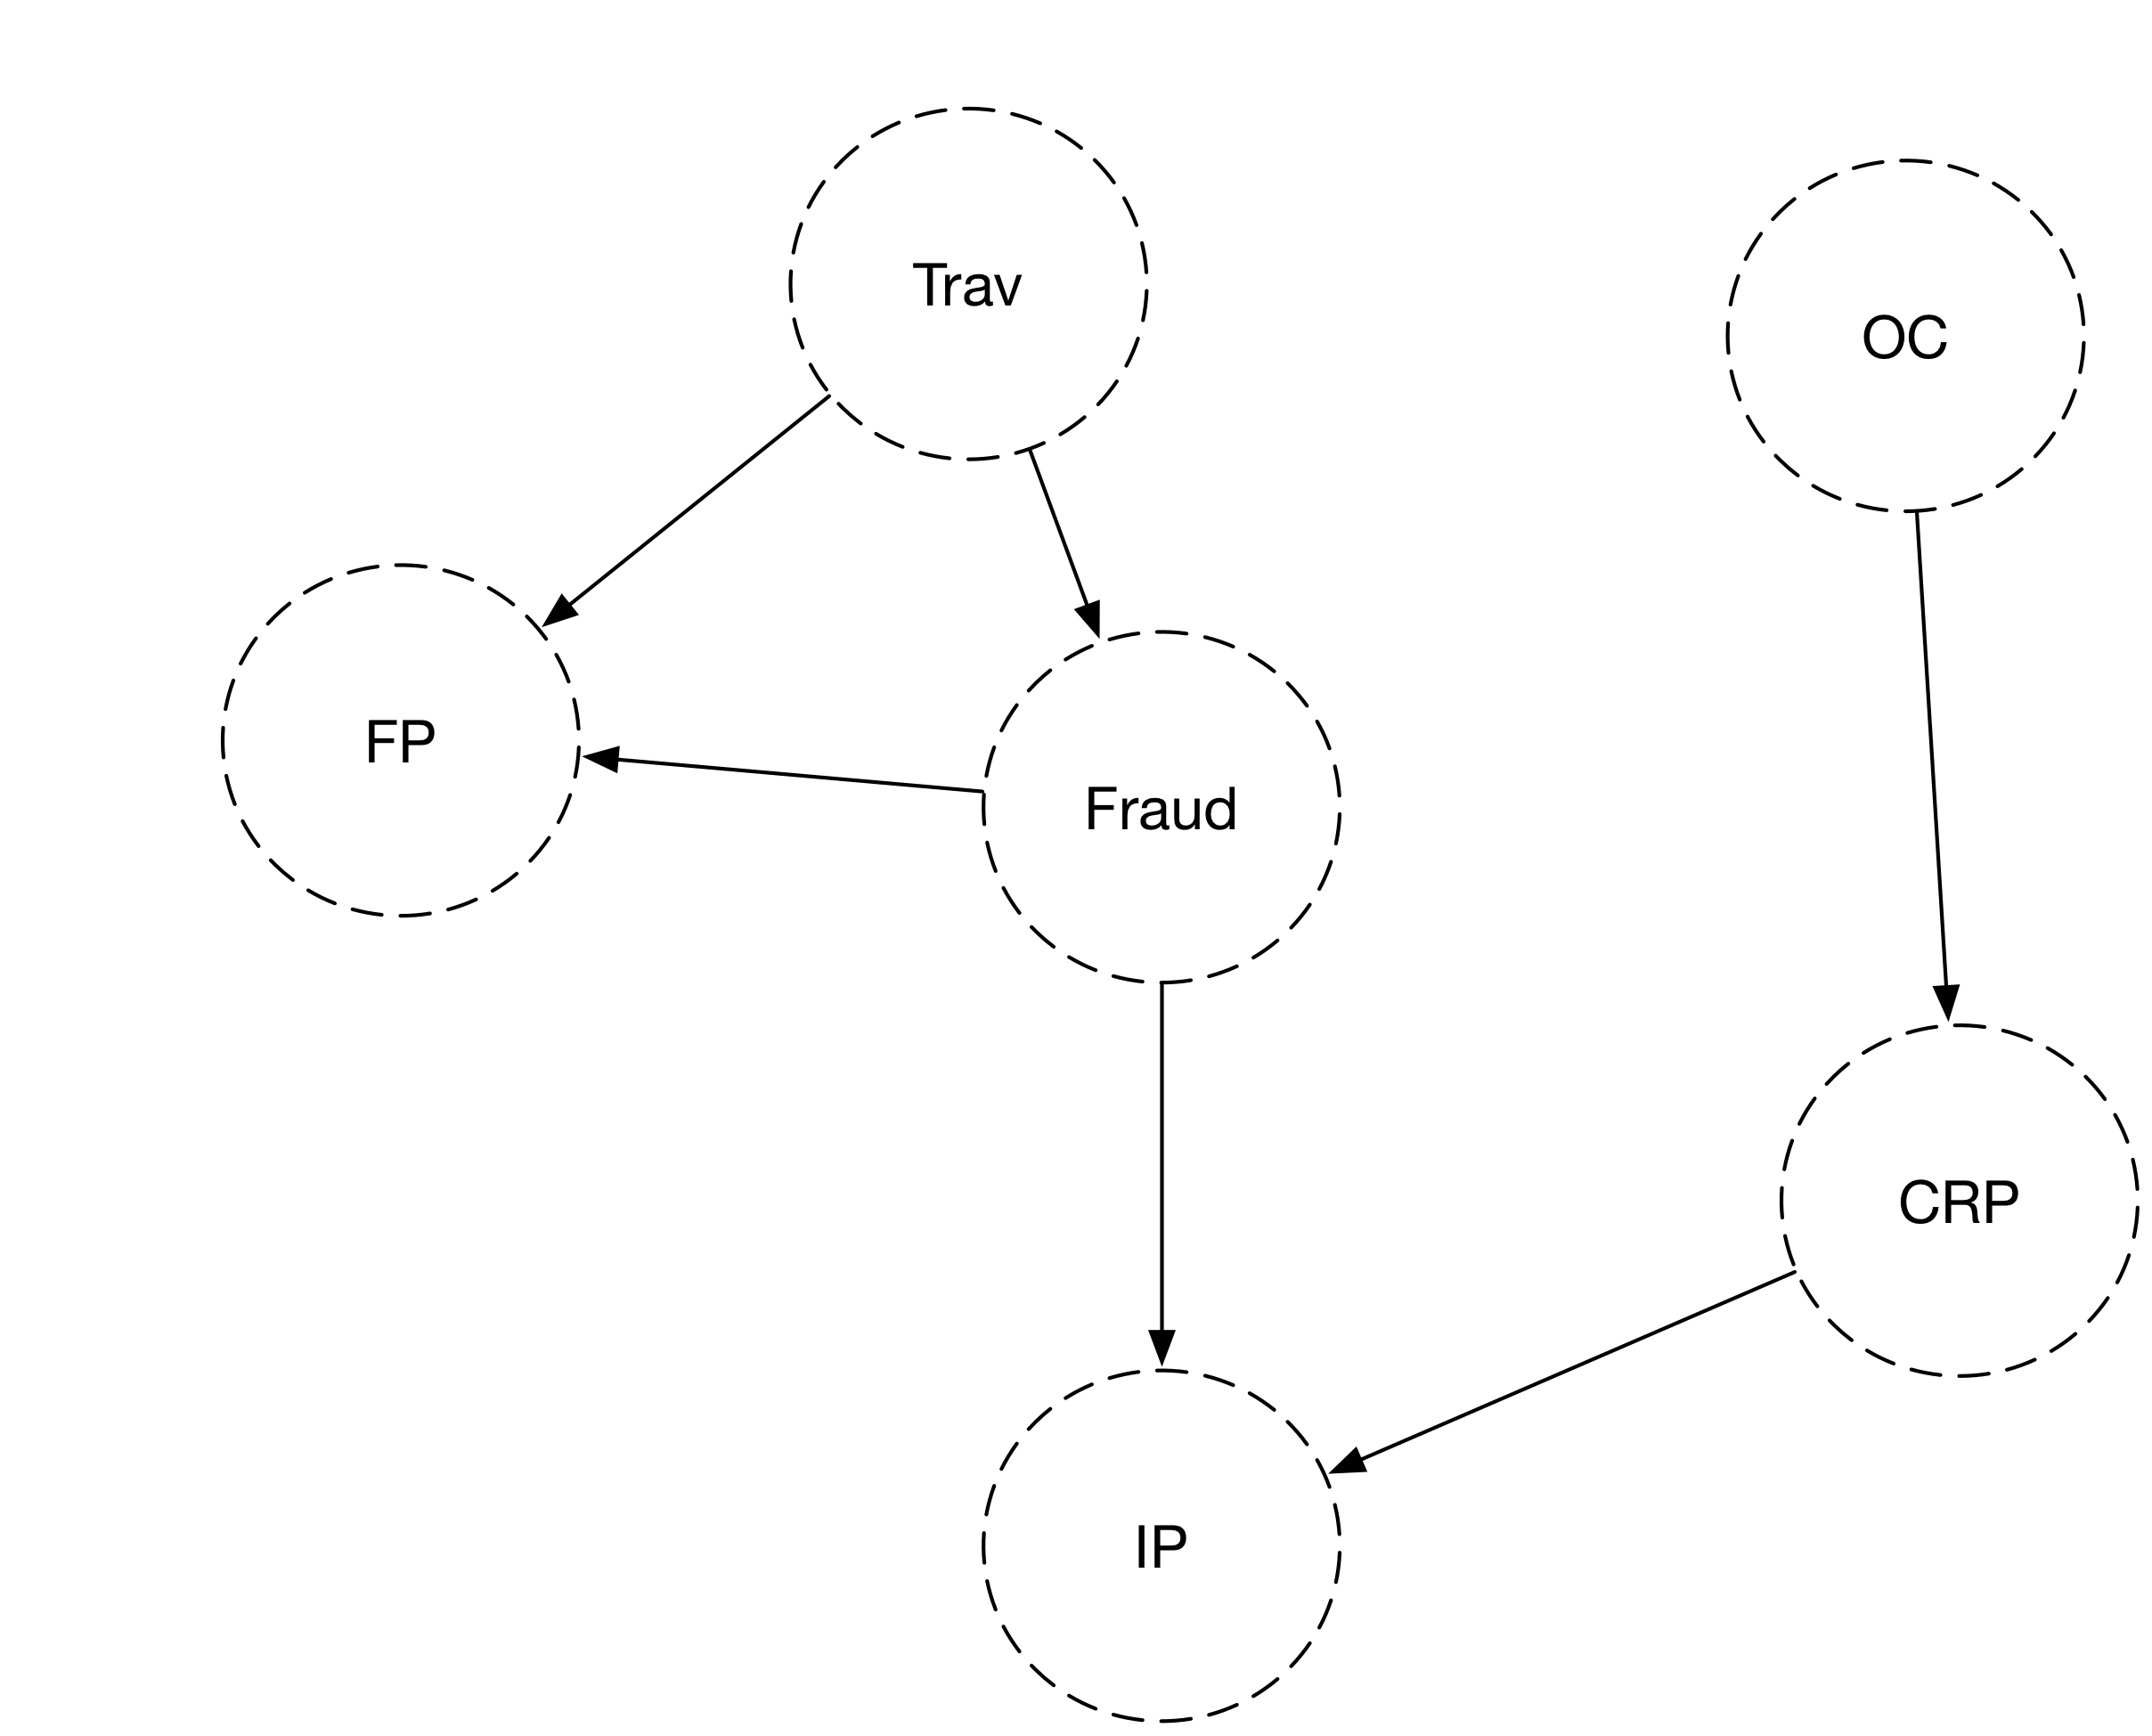
\includegraphics[width=\textwidth]{7_1.png}

\begin{table}[!hbp]
\begin{tabular}{|c|c|c|}
\hline
Trav & P  \\
\hline
True & 0.05 \\
\hline
False &  0.95\\
\hline
\end{tabular}
\caption{example of table}
\end{table} 

\begin{table}[!hbp]
\begin{tabular}{|c|c|c|}
\hline
OC & P  \\
\hline
True & 0.75 \\
\hline
False &  0.25\\
\hline
\end{tabular}
\caption{example of table}
\end{table} 

\begin{table}[!hbp]
\begin{tabular}{|c|c|c|}
\hline
CRP & OC & P  \\
\hline
True & True & 0.1 \\
\hline
True & False & 0.9\\
\hline
False & True & 0.001\\
\hline
False & False & 0.999\\
\hline
\end{tabular}
\caption{example of table}
\end{table} 

\begin{table}[!hbp]
\begin{tabular}{|c|c|c|}
\hline
Trav & Fraud & P  \\
\hline
True & True & 0.01 \\
\hline
True & False & 0.99\\
\hline
False & True & 0.004\\
\hline
False & False & 0.996\\
\hline
\end{tabular}
\caption{example of table}
\end{table} 

\begin{table}[!hbp]
\begin{tabular}{|c|c|c|c|}
\hline
Trav & Fraud & FP & P  \\
\hline
True & True & True & 0.009 \\
\hline
True & False & True & 0.891 \\
\hline
False & True & True & 0.0004 \\
\hline
False & False & True & 0.00996 \\
\hline
True & True & False & 0.991 \\
\hline
True & False & False & 0.109 \\
\hline
False & True & False & 0.9996 \\
\hline
False & False & False & 0.99004 \\
\hline
\end{tabular}
\caption{example of table}
\end{table} 

%\iffalse
%\section*{Part 3}
%\subsection*{3.1}
%Repeated Forward A*
%
%
%\subsection*{3.2}
%Repeated Backward A*
%
%
%the results show that Repeated Forward A* and Repeated Backward A* have no significant difference, they have almost the same running time and same expanded number of cells and different paths. The cause of difference of paths is that they have the same break ties rule.
%\section*{Part 4}
%The definition of Manhattan distance: The distance between two points measured along axes at right angles. If the agent only moves in four compass directions, it will only move along the axes we built, it assures that the Manhattan distances are consistent.
%
%It's known that the initial heuristic h is consistent, which means that for any initial state s,  \(h[s] \leq h[s_{succ}] + c(s, a)\) . This inequality will hold for all non-goal state s and their corresponding actions. if some action costs c(s, a) increases from c to c', and $c(s, a) \leq c'(s, a)$,   \(h[s] \leq h[s_{succ}] + c(s, a) \leq h[s_{succ}] + c'(s, a)\) , the heuristic remain consistent. The heuristic function h of state s become $h_{new}$,  $(h_{new}) = g[\bar{s}] + h[\bar{s}]  - g[s]$ and expansion. They, we can divide s into the following situations.
%
%\begin{enumerate}
%\item both s and succ(s, a) were expanded.  $(h_{new}[s]) = g[\bar{s}] + h[\bar{s}]  - g[s]$ $(h_{new}[succ(s, a)]) = g[\bar{s}] + h[\bar{s}]  - g[succ(s, a)]$, according to triangle inequality,  $ g[succ(s, a)] \leq g(s) + c(s, a)$, 
%$(h_{new}[s]) = g[\bar{s}] + h[\bar{s}] - g[s] \leq  g[\bar{s}] + h[\bar{s}] - (g[succ(s, a)] - c(s, a)$. thus $(h_{new}[s]) \leq (h_{new}[succ(s, a)]) + c(s, a)$
%\item 
%s were expanded but succ(s, a) were not expanded, $(h_{new}[s]) = g[\bar{s}] + h[\bar{s}]  - g[s]$ , $g[\bar{s}] + h[\bar{s}] \leq f[succ(s, a)]$,  $h_{new}[s] = g[\bar{s}] + h[\bar{s}]  - g[s] \leq g[succ(s, a)] + h'_{new}[succ(s, a)] -g[succ(s, a)] + c[s, a] \leq h'_{new}[succ(s, a)] +  c[s, a] $
%\item 
%both s and succ(s, a) were not expanded, $then h[s] \leq h[(succ(s, a))] + c(s, a)$
%\end{enumerate}
%\newpage
%\section*{Part 5}
%\subsection*{5.1}
%Repeated Forward A*
%
%
%\subsection*{5.2}
%Adaptive A*
%
%
%the results show that Adaptive A* expanded fewer cells than Repeated Forward A* and has less running time if the path is short enough.
%\newpage
%\section*{Part 6}
%The tree pointer can be represented as a two bit number .
%\begin{lstlisting}
%val directions = List((0, 1), (0, -1), (1, 0), (-1, 0))
%\end{lstlisting}
%It is calculated by father node coordinate minus child node coordinate.
%
%Another way is to use sparse matrix representing the maze since the quantity of blocked cells is small enough.
%\begin{lstlisting}
%sys.getsizeof(grid.array)
%10313
%\end{lstlisting}
%Python implementation of a 2-d array gridworld takes 10313 Bytes
%\begin{lstlisting}
%array = sparse.csr_matrix(array)
%sys.getsizeof(grid.array[0])
%64
%\end{lstlisting}
%Compressed Sparse Row method can be found in \emph{scipy} libray. 106 gridworlds can be stored in 4 MBytes using 2-d array.
%If gridworld is 1001*1001, it is approximately 13 gridworlds can be stored in 4 MBytes using sparse matrix.
%\fi


\end{document}